\documentclass[10pt]{article}
\usepackage[portuguese]{babel}
\usepackage[a4paper, top = 0.8in, bottom = 0.9in, left =0.6in, right = 0.6in]{geometry}
\usepackage[utf8]{inputenc}
\usepackage{fancyhdr}
\usepackage{multirow}
\usepackage{graphicx}
\usepackage{times}
\usepackage{subcaption}
\usepackage{booktabs}
\usepackage{microtype}
\usepackage{wrapfig}
\usepackage{circuitikz}
\usepackage{titlesec}
\usepackage{wrapfig}
\usepackage{caption}
\usepackage{ragged2e}
\usepackage{adjustbox}
\usepackage{float}
\usepackage{amsmath, mathtools, amssymb}
\usepackage{parskip}
\usepackage{array, makecell}
\usepackage{booktabs}
\titleformat{\section}
{\normalfont\large\bfseries}{\thesection)}{1em}{}
\titleformat{\subsection}
{\normalfont\normalsize\bfseries}{\thesubsection)}{1em}{}
\titleformat{\subsubsection}
{\normalfont\normalsize\bfseries}{\thesubsubsection)}{1em}{}


%\pretitle{\begin{center}\Huge\bfseries}

\pagestyle{fancy}
\fancyhead{}
\centering\chead{
\includegraphics[width=15cm]{imagens/unb_fga_logo_extenso.jpg}}
\lfoot{Prática de Circuitos 1 - 2019/1}
\rfoot{\textbf{Prof. Dr. Marcus V. Chaffim Costa}} %nome do rodape
\renewcommand{\footrulewidth}{1pt}

\setlength{\parskip}{0.1cm}
\author{Monitoria - 2019/2}
\title{Protocolo experimental 06}


%arrumação das tabelas

\setlength{\tabcolsep}{0.5em} % for the horizontal padding
{\renewcommand{\arraystretch}{1.2}}% for the vertical padding
\captionsetup[table]{name= \bfseries Tabela}
\numberwithin{table}{section}
\usepackage{array}
\newcolumntype{C}[1]{>{\centering\arraybackslash}m{#1}}

\aboverulesep=0cm
\belowrulesep=0cm

%configuracoes dos codigos em matlab
\usepackage{listings}
\usepackage{color} %red, green, blue, yellow, cyan, magenta, black, white
\definecolor{mygreen}{RGB}{28,172,0} % color values Red, Green, Blue
\definecolor{mylilas}{RGB}{170,55,241}

\lstset{language=Matlab,%
    %basicstyle=\color{red},
    breaklines=true,%
    morekeywords={matlab2tikz},
    keywordstyle=\color{blue},%
    morekeywords=[2]{1}, keywordstyle=[2]{\color{black}},
    identifierstyle=\color{black},%
    stringstyle=\color{mylilas},
    commentstyle=\color{mygreen},%
    showstringspaces=false,%without this there will be a symbol in the places where there is a space
    numbers=left,%
    numberstyle={\tiny \color{black}},% size of the numbers
    numbersep=9pt, % this defines how far the numbers are from the text
    emph=[1]{for,end,break},emphstyle=[1]\color{red}, %some words to emphasise
    %emph=[2]{word1,word2}, emphstyle=[2]{style},    
}

\allowdisplaybreaks


\begin{document}

\begin{center}
\vspace*{.03cm}
\Large\textbf{Experimento 9:}\\ %titulo
\Large{Circuitos com Amplificador Operacional}
\end{center}
\justify
\section{Questões pré-laboratoriais}
Considere os circuitos com amplificador operacional mostrados na Figura \ref{fig1}.

\begin{figure}[H]
	\begin{subfigure}{.33\textwidth}
		\begin{adjustbox}{width=1\textwidth}
  			\begin{circuitikz}[line width=.5pt]
  				\draw
  				(0, 0) node[op amp] (opamp) {}
        		(opamp.-) to[R , l^= $R_1$,-o] (-4, 0.5)node [left]{$V_1$}
        		(opamp.-) |- (-1, 2) to[R, l= $R_2$] (1, 2) -| (opamp.out)
        		to [short, -o] ($(opamp.out) + (.5,0)$)
        		($(opamp.out) + (.5,0)$) node [right] {$V_o$}
        
        (opamp.+)to [short] ($(opamp.+)+(0,-1)$) node [ground] {}
        
        ;
        
   			 \draw  (opamp.-) to[short,*-] ++(0,0);    
   			 \draw  (opamp.out) to[short,-*] ++(0,0);
  				
  			\end{circuitikz}
  			\end{adjustbox}
  		\caption{Circuito A}
		\label{fig:sfig1}
		\end{subfigure}
		\begin{subfigure}{.33\textwidth}
			\begin{adjustbox}{width=1\textwidth}
			\begin{circuitikz}[line width=.5pt] \draw
		(0,0) node [op amp] {}
		(-4.7,1.5) node [right] {$V_1$}
		(-4.7,.5) node [right] {$V_2$}
		(-4.7,-.5) node [right] {$V_3$}
		(-4, 1.5)	to [R, l=$R_1$,  o-] (-2,1.5)
			to [short] (-2,-.5)
		(-4, .5)	to [R, l=$R_3$, o-] (-2,.5)
		(-4, -.5)	to [R, l=$R_4$, o-] (-2,-.5)	
			to [short, -*] (-2,0.5)
			to [short, -*] (opamp.-)
			
		(opamp.+) to [short] ($(opamp.+) + (0, -1.5)$) node [ground]{}
			
		(opamp.-) |- (-1,2) to [R, l=$R_2$] (1,2) -| (opamp.out)
        	to [short, *-o] ($(opamp.out) + (1,0)$) node [right] {$V_o$}
        ;    

			\end{circuitikz}
			\end{adjustbox}
			\caption{Circuito B}
		\end{subfigure}
		\begin{subfigure}{.33\textwidth}
			\begin{adjustbox}{width=1\textwidth}
			\begin{circuitikz}[line width=.5pt]\draw
			
		(0,0) node [op amp] {}
		($(opamp.-)+(-3.2,0)$) node [right] {$V_1$}
		($(opamp.+)+(-3.2,0)$) node [right] {$V_2$}
		
		($(opamp.-)+(-2.5,0)$)	to [R, l=$R_1$, o-*] (opamp.-)

		($(opamp.+)+(-2.5,0)$)	to [R, l=$R_3$, o-] (opamp.+)
			
		(opamp.+) to [R, l=$R_4$, *-] ($(opamp.+) + (0, -2)$) node [ground]{}
			
		(opamp.-) |- (-1,2) to [R, l=$R_2$] (1,2) -| (opamp.out)
        	to [short, *-o] ($(opamp.out) + (1,0)$) node [right] {$V_o$}
        ;  
	
			\end{circuitikz}
			\end{adjustbox}
			\caption{Circuito C}
		\end{subfigure}
		
		\caption{Circuitos com Amplificador Operacional}
		\label{fig1}
\end{figure}


\subsection{Expressões Matemáticas}

Obtenha as expressões matemáticas da saída $V_o(t)$ em função das entradas e dos valores (literais) dos resistores para os
circuitos A, B e C da Figura 2.1. Quais os nomes dados a cada uma destas configurações de Amp Op?

\subsubsection{Circuito A}

\begin{figure}[H]
	\centering
\begin{circuitikz}[line width=.5pt, scale = .8, transform shape] \draw
  				(0, 0) node[op amp] (opamp) {}
        		(opamp.-) to[R , l^= $R_1$, i<=$i_1$,-o] (-4, 0.5)node [left]{$V_1$}
        		(opamp.-) |- (-1, 2) to[R, l= $R_2$, i^<=$i_2$] (1, 2) -| (opamp.out)
        		to [short, -o] ($(opamp.out) + (.5,0)$)
        		($(opamp.out) + (.5,0)$) node [right] {$V_o$}
        
        (opamp.+)to [short] ($(opamp.+)+(0,-1)$) node [ground] {}
        
        ;
        
   			 \draw  (opamp.-) to[short,*-] ++(0,0);    
   			 \draw  (opamp.out) to[short,-*] ++(0,0);
 	
\end{circuitikz}


	\caption{Amplificador Inversor}
\end{figure}


	\justify
	
	Devemos notar que as entradas do Amplificador Operacional são nulas. Dessa forma, podemos escrever a seguinte relação:
	\begin{gather*}
		i_1=i_2 
		\\
		\\
		\dfrac{0-V_1}{R_1}=\dfrac{V_o -0}{R_2}
		\Longrightarrow
		\dfrac{V_o}{R_2} = \dfrac{-V_1}{R_1}
	\end{gather*}
	
	Esse circuito é conhecido como Amplificador inversor, pois
	\begin{equation}\label{eqna}
		V_o=-\dfrac{R_2}{R_1}V_1
	\end{equation}

\subsubsection{Circuito B}




\begin{figure}[H]

	\centering
\begin{circuitikz}[line width=.5pt, scale=.8, transform shape] \draw
		(0,0) node [op amp] {}
		(-4.7,1.5) node [right] {$V_1$}
		(-4.7,.5) node [right] {$V_2$}
		(-4.7,-.5) node [right] {$V_3$}
		(-4, 1.5)	to [R, l=$R_1$, i=$i_1$, o-] (-2,1.5)
			to [short, -*] (-2,-.5)
		(-4, .5)	to [R, l=$R_3$, i=$i_2$, o-] (-2,.5)
		(-4, -.5)	to [R, l=$R_4$, i=$i_3$, o-] (-2,-.5)	
			to [short, -] (-2,0.5)
			to [short, -*] (opamp.-) node [below] {$0V$}
			
		(opamp.+) to [short] ($(opamp.+) + (0, -1.5)$) node [ground]{}
			
		(opamp.-) |- (-1,2) to [R, l=$R_2$, i^<=$i$] (1,2) -| (opamp.out)
        	to [short, *-o] ($(opamp.out) + (1,0)$) node [right] {$V_o$}
        ;    
    

\end{circuitikz}

	\caption{Amplificador Somador Inversor}
\end{figure}
	
	De mesma forma que o anterior, considerando o modelo ideal, as entradas são nulas e o ganho, infinito. Assim podemos aplicar a lei de Kirchoff:
	
	\begin{gather*}
		i = i_1 + i_2 + i_3
        \\
        \\
		\dfrac{V_o-0}{R_2}=\dfrac{0-V_1}{R_1}+\dfrac{0-V_2}{R_3} + \dfrac{0-V_3}{R_3}		
	\end{gather*}
	\begin{equation}\label{eqnb}
		V_o = - \left(\dfrac{V_1}{R_1}+\dfrac{V_2}{R_3}+\dfrac{V_3}{R_3}	\right)R_2
	\end{equation}
	Esta última explicita a propriedade soma e inversão do circuito.


\subsubsection{Circuito C}

	\begin{figure}[H]
	\centering
	
		\begin{circuitikz}[line width=.5pt, scale = .8, transform shape]\draw
		(0,0) node [op amp] {}
		($(opamp.-)+(-3.2,0)$) node [right] {$V_1$}
		($(opamp.+)+(-3.2,0)$) node [right] {$V_2$}
		
		($(opamp.-)+(-2.5,0)$)	to [R, l=$R_1$, i=$i_1$, o-*] (opamp.-) node [below] {$V_-$}

		($(opamp.+)+(-2.5,0)$)	to [R, l=$R_3$, o-] (opamp.+) node [above] {$V_+$}	
			
		(opamp.+) to [R, l=$R_4$, *-] ($(opamp.+) + (0, -2)$) node [ground]{}
			
		(opamp.-) |- (-1,2) to [R, l=$R_2$, i=$i_2$] (1,2) -| (opamp.out)
        	to [short, *-o] ($(opamp.out) + (1,0)$) node [right] {$V_o$}
        ;  
	\end{circuitikz}

	\caption{Circuito Subtrator}
	\end{figure}

	Considerando as condições ideais, construa a lei de Kirchhoff para as tensões referente ao nó da entrada inversora e da entrada não inversora:
	
	\begin{gather*}	
		i_1 = i_2
		\\
		\\
		\dfrac{V_- - V_1}{R_1}= \dfrac{V_o - V_-}{R_2}
        \Longrightarrow
		\dfrac{V_-}{R_1} + \dfrac{V_-}{R_2} = \dfrac{V_o}{R_2} + \dfrac{V_1}{R_1}
	\end{gather*}
	\\
	\begin{equation} \label{3_1}
		\left(\dfrac{1}{R_1} + \dfrac{1}{R_2}\right)V_- = \dfrac{V_o}{R_2} + \dfrac{V_1}{R_1}
	\end{equation}
		Nesse ponto, necessitamos encontrar um valor que relacione os resistores $R_3$ e $R_4$. Notando que $V_-=V_+$, calcularemos a expressão para o nó $V_+$:

%\begin{minipage}{.4\linewidth}
	\begin{gather*}
		V_-=V_+
		\\
		\\
		\dfrac{V_+ -V_2}{R_3}+\dfrac{V_+ - 0}{R_4} = 0
        \Longrightarrow
		\dfrac{V_+}{R_3} + \dfrac{V_+}{R_4} = \dfrac{V_2}{R_3}
		\Longrightarrow
		\left(\dfrac{1}{R_3 + R_4}\right) V_+ = \dfrac{V_2}{R_3}
	\end{gather*}
	\\
	\begin{equation}\label{eqn3_2}
		V_+ = \left(\dfrac{R_3 R_4}{R_3 + R_4}\right) \dfrac{V_2}{R_3}
	\end{equation}
%\end{minipage}
%\begin{minipage}{.5\linewidth}
	Substituindo \ref{eqn3_2} em \ref{3_1}, temos
	\\
	\begin{equation*}
	\left(\dfrac{R_1+R_2}{R_1 R_2}\right)\left(\dfrac{R_3 R_4}{R_3 + R_4}\right)\dfrac{V_2}{R_3} = \dfrac{V_o}{R_2} + \dfrac{V_1}{R_1}
	\end{equation*}
	\\
	Isolando o $\dfrac{V_o}{R_2}$, obtemos
	\\
	\begin{equation*}
		\left(\dfrac{R_1+R_2}{R_1 R_2}\right)\left(\dfrac{R_3 R_4}{R_3 + R_4}\right)\dfrac{V_2}{R_3} - \dfrac{V_1}{R_1} = \dfrac{V_o}{R_2}
	\end{equation*}
	\\
	\begin{equation}
		V_o = \left(\dfrac{R_1+R_2}{R_1 R_2}\right)\left(\dfrac{R_3 R_4}{R_3 + R_4}\right)\dfrac{R_2}{R_3} V_2 - \dfrac{R_2}{R_1}V_1
	\end{equation}
	
%\end{minipage}
\section{Circuitos Integrados com Amplificadores Operacionais}
\label{sec:circuitos_integrados}
Temos disponíveis no repositório 3 modelos de CI portador de amplificador operacional: \textbf{uA741, LM358 e LM324}. As peculiaridades de cada um serão descritas no fio abaixo, respectivamente:
\begin{enumerate}
    \item O CI uA741 possui apenas um amplificador operacional. Possui entradas de ajuste de \emph{offset}, para eliminar as variações de tensão entre as entradas inversora e não inversora do amplificador operacional. A alimentação é feita a partir de uma alimentação $V_{cc+}$ e $V_{cc-}$, onde ambos os valores devem ser iguais, com o sinal oposto. A disposição dos pinos do CI estão na figura \ref{fig:ua741}.
    \begin{figure}[H]
        \centering
        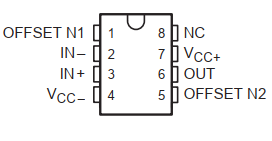
\includegraphics{imagens/ua741.png}
        \caption{Pinagem do CI uA741}
        \label{fig:ua741}
    \end{figure}
    
    \item O LM358 possui dois amplificadores operacionais, A e B. Eles não possuem ajuste de \emph{offset}. A alimentação é feita de dois modos: alimentando $V^+$ com 3V até 32V e GND aterrado, ou alimentando $V^+$ com +1.5V até +16V e GND com -1.5V até -16V, ambas as alimentações das entradas devem ser idênticas com sinais opostos. O arranjo dos pinos está disposto na figura \ref{fig:lm358}.
    \begin{figure}[H]
        \centering
        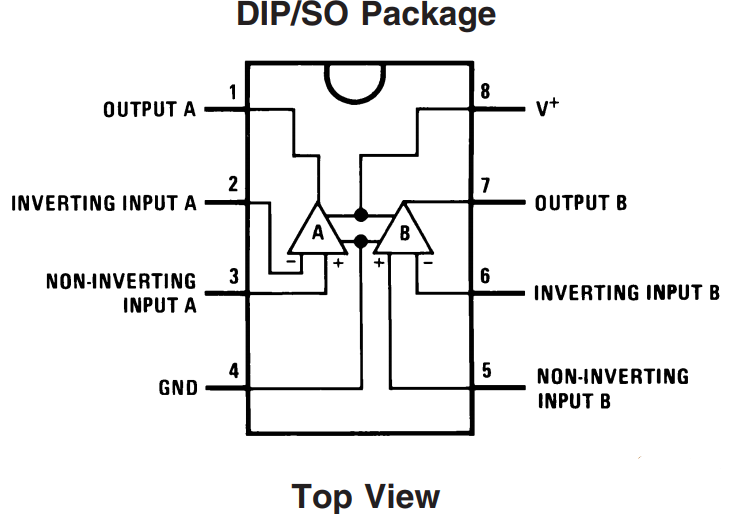
\includegraphics[width=.4\linewidth]{imagens/LM358.png}
        \caption{Pinagem do CI LM358}
        \label{fig:lm358}
    \end{figure}
    
    \item O terceiro CI, LM324, se dispõe de quatro amplificadores operacionais. Também não possui ajuste de \emph{offset}. A alimentação é feita da mesma forma que o CI LM 358. A pinagem utilizada é mostrada na figura \ref{fig:lm324}.
    \begin{figure}[H]
        \centering
        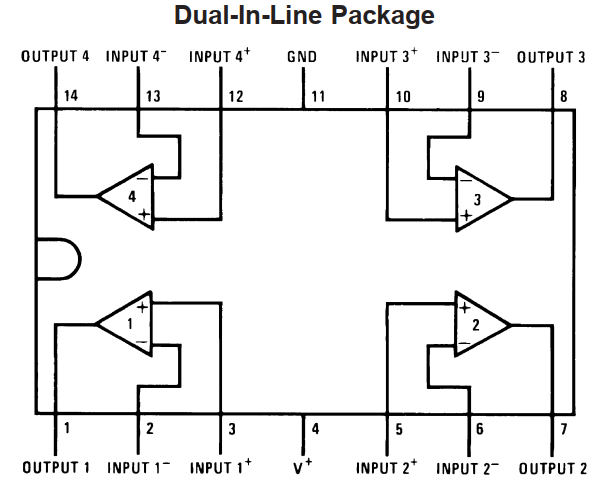
\includegraphics[width=.4\linewidth]{imagens/LM324.png}
        \caption{Pinagem do CI LM324}
        \label{fig:lm324}
    \end{figure}
\end{enumerate}

\section{Efeitos limitadores dos amplificadores operacionais}

O conhecimento de uma série de parâmetros dos amplificadores operacionais reais são determinísticos para a compreensão do seu desempenho. O fio abaixo mostra os principais deles:

\begin{itemize}
    \item \textbf{Ganho Finito:} é a relação do ganho de tensão na saída em relação a entrada, a partir da variação de tensão nos terminais positivo e negativo do amplificador operacional. Desse modo, nós obtemos a relação $A(V^+ - V^-)=V_o$, onde A caracteriza o ganho, podendo chegar a casa de dezenas de milhares de unidades.
    
    \item \textbf{Impedância de entrada finita:} o modelo ideal de amplificador operacional assume que temos corrente zero passando pelos terminais. Entretanto, essa impedância de entrada é limitada quando medido a resistência de um dos terminais com o outro aterrado, ainda que esta seja na casa dos milhões de Ohms.
    
    \item \textbf{Tensão de \emph{offset} de entrada:} devido as diferenças mínimas de fabricação de cada componente do amplificador operacional, a saída do amplificador operacional não obedecerá o modelo ideal, \textit{i.e.}, terá sua saída com tensão diferente de zero. Pode-se perceber esse efeito ao aterrar ambas as entradas do amplificador operacional e medir a sua saída. Geralmente, esse \emph{offset} é ignorado por ser quase insignificante em alguns casos.
    
    \item \textbf{Lagura de banda finita:} os amplificadores operacionais possuem uma resposta em frequência do tipo passa-baixa. O efeito é causado principalmente por conta dos capacitores envolvidos no circuito do amplificador, fazendo com que a amplitude do sinal de saída diminua a partir das faixas mais altas de frequência.
    
    \item \textbf{Capacitância de entrada:} é a capacitância oferecida pelo amplificador operacional real, diferindo do modelo ideal que é zero. Ela é a responsável pelo comportamento do circuito em frequências altas.
    
    \item \textbf{Saturação:} A tensão de saída é limitada inferior e superiormente por um limiar de saturação, que é atingido um pouco antes dos valores de alimentação do amplificador operacional. Esse limiar é definido no projeto quando configurado as tensões de alimentação \cite{dorf}.
    
    \item \textbf{\emph{Slew-rate}:} é a taxa em que a tensão de saída consegue variar em $\mu s$ em relação a entrada. A imperfeição se deve aos condensadores presentes no componentes, uma vez que a resposta em frequência da tensão dos capacitores não é imediata.
\end{itemize}
\section{Impedâncias}

\subsection{Circuito A}
A figura \ref{fig:circuit_a_imp} retrata o modelo de impedância de entrada para o circuito Amplificador Operacional Inversor.

\begin{figure}[H] 
    \centering
    \begin{adjustbox}{width=.5\textwidth}
    \begin{circuitikz}[line width=.5pt]
        \draw
        
        (0,0) node [ground] {} to [american controlled voltage source , l_= $A(V^+-V^-)$, invert] (0,3)
            to [R = $R_o$, -o] (5,3) node [right] {$V_o$}
            (4,3) to [short, *-] (4,5)
            to [R=$R_2$, f<=$i_2$] (-4,5)
            to [short, -*] (-4,3)
            to [R = $R_1$, f<=$i_1$, -o] (-7,3)
            (-7.7,3) node[right] {$V_1$}
            
            (-4,3) to [short, f=$i_i$] (-2,3)
            to [R = $R_i$] (-2,1)
            to [short] (-4,1)
            to [short] (-4,0) 
            to [short,-*] (0,0)
            to [short, -*] (3,0)
            
        ;
            
    \end{circuitikz}
    \end{adjustbox}
    \caption{Circuito A}
    \label{fig:circuit_a_imp}
\end{figure}

Podemos aplicar a Lei de Kirchhoff no nó de entrada para observar o comportamento da resistência de entrada:

    

\begin{gather*}
    i_1 =i_2+i_i\\\\
    \dfrac{V_- - V_1}{R_1} = \dfrac{V_o - V_-}{R_2} + \dfrac{V_+ - V_-}{R_i}
    \Longrightarrow
    \dfrac{V_+ - V_-}{R_i} = \dfrac{ V_- - V_1}{R_1} - \dfrac{V_o - V_-}{R_2}
    \\
    \\
    \dfrac{V_+ - V_-}{R_i} = \dfrac{(V_- - V_1)R_2 - (V_o - V_-)R_1}{R_1 R_2}\\
\end{gather*}
\begin{equation}
    R_i = \dfrac{(V_+ - V_-) R_1 R_2}{(V_- - V_1) R_2 - (V_o - V_-)R_1}
\end{equation}

Para a resistência de saída, aplicamos a Lei de Kirchhoff no nó de saída, donde obtemos

\begin{gather*}
    \dfrac{V_o - V_-}{R_2} = \dfrac{A(V_+ - V_-) - V_o}{R_o}
\end{gather*}
\begin{equation}
        R_o = \dfrac{(AV_+ - AV_- - V_o)R_2}{V_o - V_-}
\end{equation}

\subsection{Circuito B}

    O circuito da figura \ref{fig:circuit_b_imp} retrata o modelo de circuito Amplificador Operacional Somador Inverso.

\begin{figure}[H]
    \centering
    \begin{adjustbox}{width=.5\textwidth}
    \begin{circuitikz}[line width = .5pt]
        \draw
            (0,0) node [ground] {} to [american controlled voltage source , l_= $A(V^+-V^-)$, invert] (0,3)
            to [R = $R_o$, -o] (5,3) node [right] {$V_o$}
            (4,3) to [short, *-] (4,5)
            to [R=$R_2$, f<^=$i$] (-4,5)
            to [short, -*] (-4,3) -- (-5,3)
            to [R = $R_3$, f<=$i_2$, -o] (-8,3)
            node[left] {$V_2$}
            (-5,3) to [short,*-] (-5,4)
            to [R = $R_1$, f<=$i_2$, -o] (-8,4) node [left] {$V_1$}
            (-5,3) to [short] (-5,2)
            to [R = $R_4$, f<=$i_3$, -o] (-8,2) node [left] {$V_3$}
            
            (-4,3) to [short, f=$i_i$] (-2,3)
            to [R = $R_i$] (-2,1)
            to [short] (-4,1)
            to [short] (-4,0) 
            to [short,-*] (0,0)
            to [short, -*] (3,0)
            
        ;
    \end{circuitikz}
    \end{adjustbox}
    \caption{Circuito B}
    \label{fig:circuit_b_imp}
\end{figure}

    Podemos observar o comportamento da impedância de entrada analisando o nó de entrada com a Lei de Kirchhoff:
    
    \begin{gather*}
        i + i_i = i_1 + i_2 + i_3\\ \\
        \dfrac{V_o - V_-}{R_2} + \dfrac{V_+ - V_-}{R_i} = \dfrac{V_- - V_1}{R_1} + \dfrac{V_- - V_2}{R_3} + \dfrac{V_- - V_3}{R_4}\\
        \dfrac{V_+ - V_-}{R_i} = \dfrac{V_- - V_1}{R_1} + \dfrac{V_- -V_2}{R_3} + \dfrac{V_- -V_3}{R_4} - \dfrac{V_o - V_-}{R_2}\\
        \dfrac{V_+ - V_-}{R_i} = \dfrac{(V_- - V_1)R_2 R_3 R_4 - (V_o - V_-)R_1 R_3 R_4 + (V_- - V_2)R_1 R_2 R_4 + (V_- - V_3)R_1 R_2 R_3}{R_1 R_2 R_3 R_4}\\
        R_i=\dfrac{R_1 R_2 R_3 R_4(V_+ - V_-)}{(V_- - V_1)R_2 R_3 R_4 - (V_o - V_-)R_1 R_3 R_4 + (V_- - V_2)R_1 R_2 R_4 + (V_- - V_3)R_1 R_2 R_3}
    \end{gather*}
    
    Podemos analisar a impedância de saída a partir do nó de saída do circuito, donde temos
    \begin{gather*}
        \dfrac{V_o - V_-}{R_2} = \dfrac{A(V_+ - V_-) - V_o}{R_o}\\
        R_o = \dfrac{(AV_+ - AV_- - V_o)R_2}{V_o - V_-}
    \end{gather*}

\subsection{Circuito C}

\begin{figure}[H]
    \centering
    \begin{adjustbox}{width=.5\textwidth}
    \begin{circuitikz}[line width = .5pt]
        \draw
            (0,0) node [ground] {} to [american controlled voltage source , l_= $A(V^+-V^-)$, invert] (0,3)
            to [R = $R_o$, -o] (5,3) node [right] {$V_o$}
            (4,3) to [short, *-] (4,6)
            to [R=$R_2$, f<^=$i_2$] (-4,6)
            to [short, -*] (-4,4.5)
            to [R = $R_1$, f<=$i_1$, -o] (-8,4.5)
            node[left] {$V_1$}
            (-8,2.5) node [left] {$V_2$}
            to [R = $R_3$, f>^=$i_3$, o-*] (-4,2.5)
            
            (-4,4.5) to [short, f=$i_i$] (-2,4.5)
            to [R = $R_i$] (-2,2.5)
            to [short] (-4,2.5)
            to [R = $R_4$, f_= $i_4$](-4,0)
            to [short,-*] (0,0)
            to [short, -*] (3,0)
            
        ;
    \end{circuitikz}
    \end{adjustbox}
    \caption{Circuito C}
    \label{fig:circuit_c_imp}
\end{figure}

 O circuito da figura \ref{fig:circuit_c_imp} é uma abstração do funcionamento do amplificador operacional arranjado na configuração de Subtrator.
 
 Analisando o nó de entrada, podemos obter a impedância de entrada. Desse modo, 
 
\begin{gather*}
     i_i = i_2 - i_1\\ \\
     \dfrac{V_+ - V_-}{R_i} = \dfrac{V_o - V_-}{R_2} - \dfrac{V_- - V_1}{R_1}
\end{gather*}
\begin{equation}
         R_i = \dfrac{(V_+ - V_-)R_1 R_2}{(V_o - V_-)R_1 - (V_- - V_1)R_2}
\end{equation}
\begin{center}
    ou
\end{center}
\begin{gather*}
     i_i = i_4 - i_3\\
     \\
     \dfrac{V_+-V_-}{R_i} = \dfrac{V_o - V_-}{R_4} - \dfrac{V_- - V_2}{R_3}\\
\end{gather*}
\begin{equation}
         R_i = \dfrac{(V_+ - V_-)R_3 R_4}{V_+ R_3 - (V_+ - V_2)R_4}
\end{equation}

 Agora, analisando o nó de saída, temos:
\begin{gather*}
    \dfrac{V_o - V_-}{R_2} = \dfrac{A(V_+ - V_-) - V_o}{R_o}\\
    R_o = \dfrac{(AV_+ - AV_- -V_o)R_2}{V_o - V_-}
\end{gather*}

\section{Simulações}
Para senóides com $f =100 Hz$ e resistores (em Ohms), respectivamente, $R_1 = 100\Omega$, $R_2 = 560\Omega$, $R_3 = 220\Omega$ e $R_4 = 330\Omega$, simule os circuitos A, B e C para todas as combinações de V1, V2 e V3 apresentadas na \textbf{Tabela 1} da \textbf{Folha de Dados}.

\subsection{Circuito A}


\begin{itemize}
    \item Inicialmente, abra o QUCS, vá em \textit{Main Dock} e crie uma nova pasta de projeto. 
    
    \item Na aba Componentes (\textit{Components}), vá em componentes não lineares (\textit{non linar components}) e clique em um Amplificador Operacional (\textit{OpAmp}). Em componentes agrupados (\textit{lumped components}) e clique em dois resistores. Vá em Fontes (\textit{sources}) e coloque uma fonte de tensão AC (\textit{AC voltage Source}).
\end{itemize}

\begin{figure}[H]
    \begin{subfigure}{.4\textwidth}
        \centering
        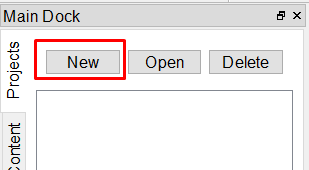
\includegraphics[width=.7\textwidth]{imagens/CircuitoA/new.png}
        \caption{Criação de um novo Projeto}
        \label{fig:new_proj}
    \end{subfigure}    
    \begin{subfigure}{.4\textwidth}
        \centering
        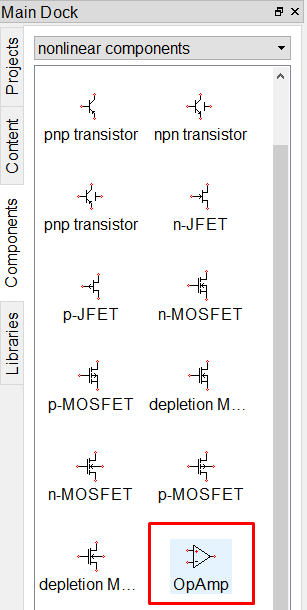
\includegraphics[width=.7\textwidth, trim={ 0 0 0 9cm}, clip]{imagens/CircuitoA/OpAmp.png}
        \caption{Seleção do Amp Op.}
        \label{fig:sel_ampop}
    \end{subfigure}
    
    \begin{subfigure}{.4\textwidth}
        \centering
        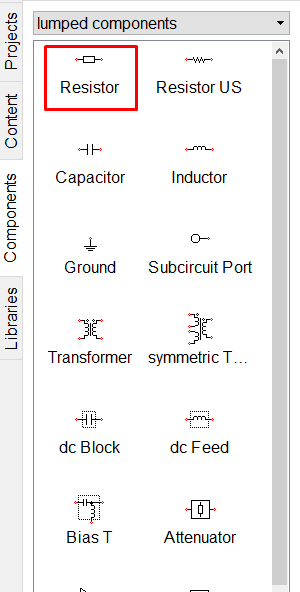
\includegraphics[width=.7\textwidth,  trim={0 7cm 0 0}, clip]{imagens/CircuitoA/resistor.png}
        \caption{Seleção do Resistor.}
        \label{fig:sel_res}
    \end{subfigure}
    \begin{subfigure}{.4\textwidth}
        \centering
        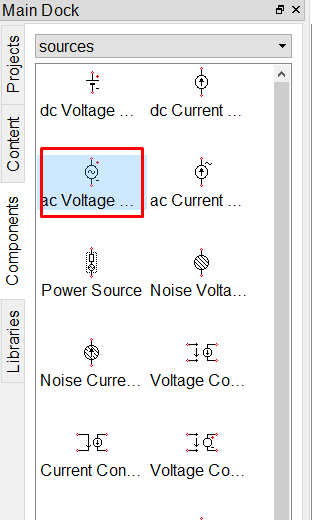
\includegraphics[width=.7\textwidth,  trim={0 7cm 0 0}, clip]{imagens/CircuitoA/fonto_ac.png}
        \caption{Seleção da fonte AC}
        \label{fig:new_proj}
    \end{subfigure}

    \caption{Abertura do projeto e seleção dos componentes }
\end{figure}

\begin{itemize}
    \item Conecte os componentes como a figura \ref{fig:circ_a_q}. Não se esqueça da referência e ajustar os valores dos resistores.
    \item É importante salientar que para essa simulação, necessitaremos de uma simulação AC e outra DC. A simulação AC é necessária para a fonte de voltagem AC, enquanto a fonte DC tem sua utilidade na ligação DC do Amplificador Operacional, \textit{i.e.}, tem seu efeito na energização do $V_{dd}$ e $V_{ss}$ do Amp Op.
    \item  Configure a Simulação AC para observar o valor da saída para a frequência desejada. Salve e simule.
    \item Vá em \textit{Diagramas} e insira uma tabela. Coloque o valor da tensão $V_o.v$. O resultado final deve ser igual ao representado na Figura \ref{fig:circ_a_q}.
    
    \begin{figure}[H]
        \centering
        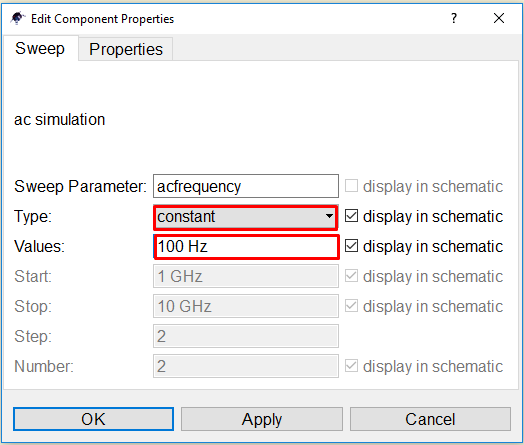
\includegraphics[width=.5\textwidth]{imagens/CircuitoA/simulacao.png}
        \caption{Parâmetros de Simulação AC.}
        \label{fig:my_label}
    \end{figure}
    
\end{itemize}


\begin{figure}[H]
    \centering
    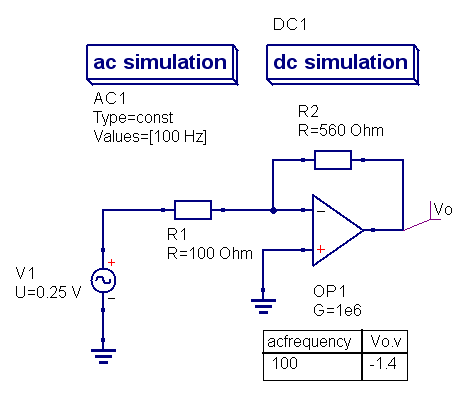
\includegraphics[width=.5\textwidth]{imagens/CircuitoA/circuito_a_sim.png}
    \caption{Arranjo do Circuito A no QUCS.}
    \label{fig:circ_a_q}
\end{figure}

\subsection{Circuito B}
    \begin{itemize}
        \item Vá em arquivo e clique em \textit{Salvar como} e mude o nome do arquivo para utilizar o esquemático já montado para o próximo circuito.
        \item Na aba \textit{Componentes}, vá em componentes agrupados e coloque mais dois resistores. Vá em Fontes e coloque mais duas fontes de tensão AC.
        \item Há duas formas de gerar os circuitos: gerar um por vez, cada qual com seu arquivo; gerar todos de uma só vez, num único arquivo (recomendado).
        \item Nesse tutorial, foi feito todas as variações da tabela 1 da folha de dados em um esquemáticos distintos, como ilustrado nas figuras \ref{fig:2_fon_des}, \ref{fig:1_fon_des} e \ref{fig:0_fon_des}.
    \end{itemize}

\begin{figure}[H]
   
    \begin{subfigure}{.4\textwidth}
        \centering
        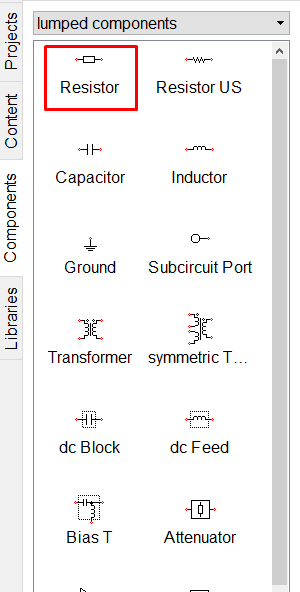
\includegraphics[width=.7\textwidth, trim={0 9cm 0 0}, clip]{imagens/CircuitoA/resistor.png}
        \caption{Seleção dos Resistores}
        \label{fig:sel_resis}
    \end{subfigure}
    \begin{subfigure}{.4\textwidth}
        \centering
        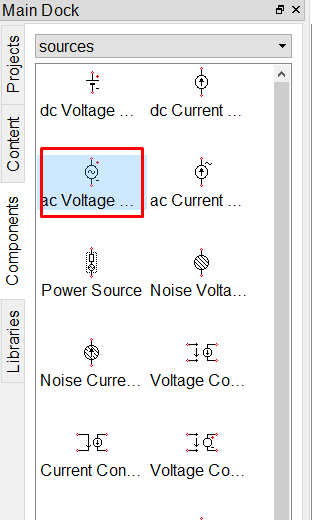
\includegraphics[width=.7\textwidth, trim={0 7cm 0 0}, clip]{imagens/CircuitoA/fonto_ac.png}
        \caption{Seleção fonte AC}
        \label{fig:sel_font_ac}
    \end{subfigure}    
    
 \begin{subfigure}{.45\textwidth}
        \centering
        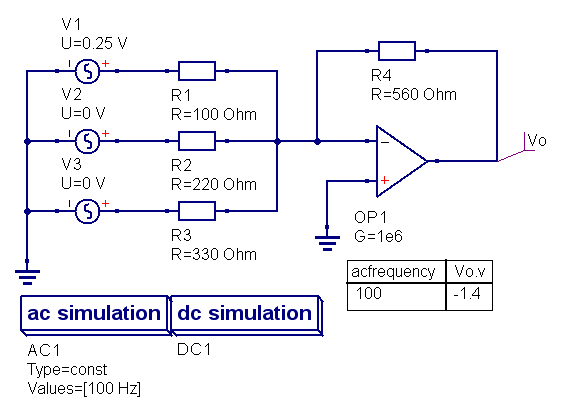
\includegraphics[width=\textwidth]{imagens/CircuitoB/-1_4.png}
        \caption{Uma fonte desativada}
        \label{fig:2_fon_des}
    \end{subfigure}    
    \begin{subfigure}{.45\textwidth}
        \centering
        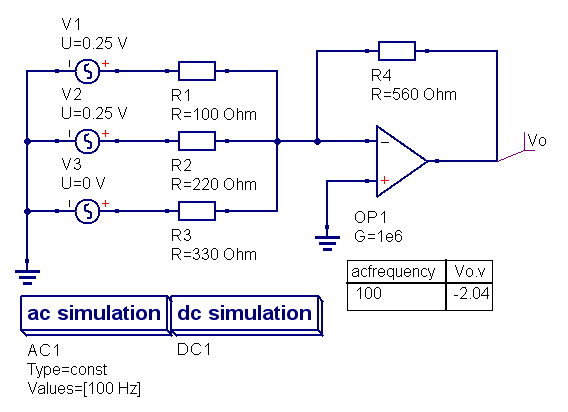
\includegraphics[width=\textwidth]{imagens/CircuitoB/-2_04.png}
        \caption{Apenas uma fonte desativada}
        \label{fig:1_fon_des}
    \end{subfigure}
    \centering
    \begin{subfigure}{.45\textwidth}
        \centering
        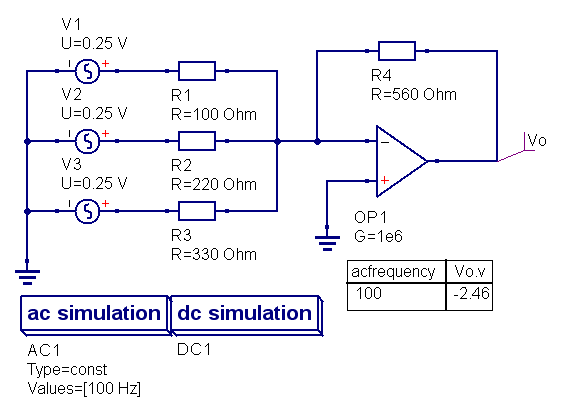
\includegraphics[width=\textwidth]{imagens/CircuitoB/-2_46.png}
        \caption{Todas as fontes Ativas}
        \label{fig:0_fon_des}
     \end{subfigure}
\end{figure}



\subsection{Circuito C}


    \begin{itemize}
        \item Vá em Arquivo e depois em Salvar como... e mude o nome do arquivo para utilizar o esquemático já montado para a o próximo circuito. Exclua a Fonte $V_3$ e conecte os componentes sem esquecer da referência do terra.
        \item Copie  e cole o circuito e modifique os valores das fontes para $V_1 = 0,5V_{pp}$ e $V_2=0V_{pp}$.
        \item Copie e cole em outro espaço, novamente, e modifique os valores das fontes para $V_1 = 0V_{pp}$ e $V_2=0,5V_{pp}$.
        \item Salve e simule.
        \item Vá em Diagramas e insira uma tabela. Coloque o valor das tensões.
        \item Nesse ponto do tutorial, foi colocado todos os circuitos em um único esquemático.
        \item O resultado obtido deve ser semelhante ao apresentado na figura \ref{fig:circuito_c_sim}.
    \end{itemize}

    \begin{figure}[H]
        \centering
        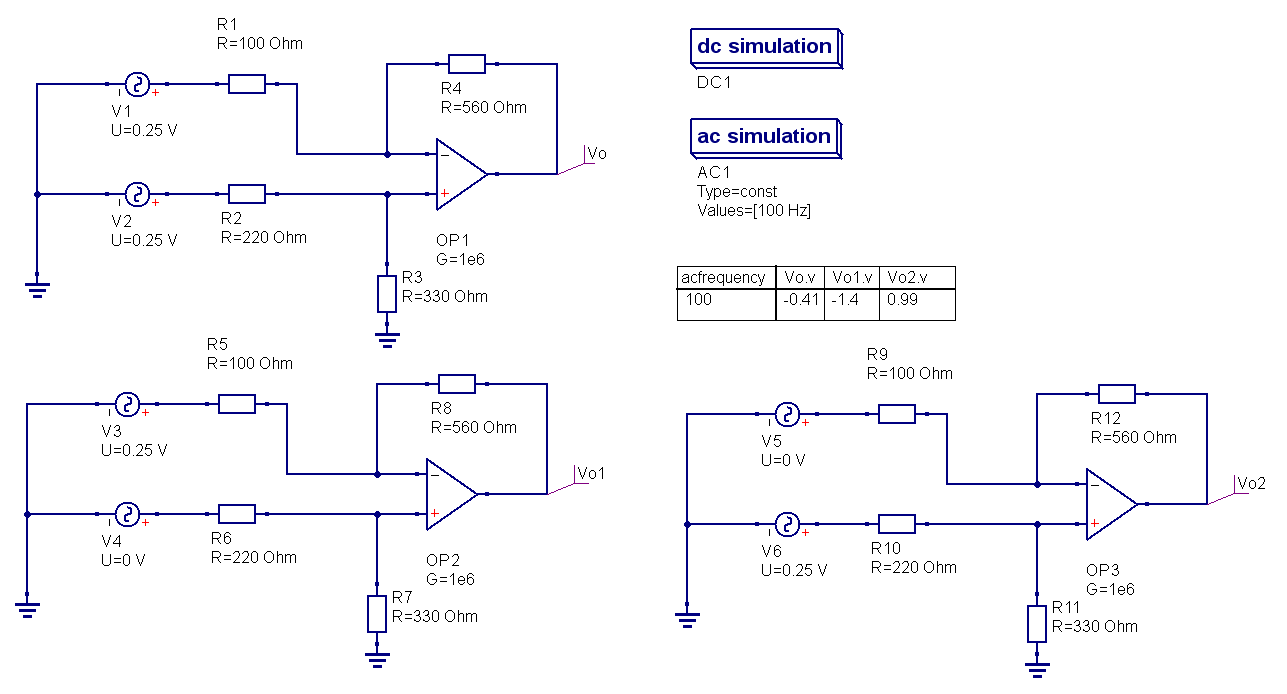
\includegraphics[width=\textwidth]{imagens/CircuitoC/sim_c.png}
        \caption{Esquemático do circuito montado}
        \label{fig:circuito_c_sim}
    \end{figure}
\section{Experimento}

\subsection{Caracterização de circuitos com resistores e Amplificador
Operacional}

Monte cada um dos circuitos das figuras A, B e C, com tensões de alimentação
$V_{ss}=-10\textrm{V}$ e $V_{dd}=+10\textrm{V}$. Utilize os valores
definidos pelo professor para $R_{1}$, $R_{2}$, $R_{3}$ e $R_{4}$.
Estabeleça experimentalmente a relação entre as amplitudes pico-a-pico
dos sinais de entrada $V_{1}(t)$, $V_{2}(t)$ e $V_{3}(t)$ e a amplitude
pico-a-pico do sinal de saída $V_{o}(t)$ observados no osciloscópio.
Use o gerador de funções nas entradas, com sinais senoidais de amplitudes
definidas segundo a Tabela 1 da Folha de Dados, e com a frequência
arbitrada pelo professor. 

Meça com precisão os valores das resistências $R_{1}$, $R_{2}$,
$R_{3}$ e $R_{4}$ com um multímetro e substitua estes valores nas
expressões obtidas no item 2.1. Compare os resultados experimentais
com os valores teóricos para o ganho de tensão de cada circuito e
de cada configuração mostrados na Tabela 1 da Folha de Dados.

\subsection{Efeitos não-lineares}

\textbf{a) Slew-rate:} Determine a maior taxa de variação da tensão
por unidade de tempo $(\delta V(t)/dt)$ na saída do circuito A. Utilize
uma entrada quadrada com grande amplitude e frequência. 

\noindent\textbf{b) Saturação:} Verifique qual é a amplitude máxima de excursão
da tensão de saída $V_{o}(t)$ do circuito A. Que fatores limitam
na prática a excursão da tensão de saída? Use uma grande amplitude
de entrada, em baixa-frequência $(f<1\,\textrm{kHz})$.

\subsection{Resposta em frequência}

Usando a configuração do circuito A, aumente gradativamente a frequência
do sinal de entrada até o limite do gerador (circuito A) e anote os
valores correspondentes de ganho. Explique o comportamento do ganho
em função da frequência. Use uma entrada com pequena amplitude, para
que não ocorra influência significativa do slew-rate.

\newpage
\begin{center}
    \Large \bfseries 119148 – Prática de Circuitos Eletrônicos 1 – Folha de Dados
\end{center}

\vspace{.5cm}

\setlength{\parindent}{0.0cm}

\makebox[.3\textwidth][l]{Turma:\enspace\rule{2cm}{0.4pt}}
\makebox[.3\textwidth][l]{Bancada:\enspace\rule{2cm}{.4pt}}
\makebox[.3\textwidth][l]{Data:\enspace\rule{1cm}{.4pt}/\rule{1cm}{.4pt}/\rule{1cm}{.4pt}}
\\
\\
\makebox[.7\textwidth][l]{Nome:\enspace\rule{.6\textwidth}{0.4pt}}
\makebox[.5\textwidth][l]{Matrícula:\enspace\rule{1cm}{.4pt}/\rule{2cm}{.4 pt}}

\vspace*{5mm}
\begin{center}
    \large \bfseries Experimento 09: Circuitos com Amplificador Operacional
\end{center}
\vspace{5mm}

Resistores usados:
\\
\\
\begin{center}
$R_{1}=$\enspace \rule{1.8cm}{.4pt}\enspace$\pm$\enspace\rule{1.8cm}{.4pt}\enspace$[\Omega]$\hspace{1cm}$R_{2}=$\enspace \rule{1.8cm}{.4pt}\enspace$\pm$\enspace \rule{1.8cm}{.4pt}\enspace$[\Omega]$
\par\end{center}
\begin{center}
$R_{3}=$\enspace \rule{1.8cm}{.4pt}\enspace$\pm$\enspace\rule{1.8cm}{.4pt}\enspace$[\Omega]$\hspace{1cm}$R_{4}=$\enspace\rule{1.8cm}{.4pt}\enspace$\pm$\enspace \rule{1.8cm}{.4pt}\enspace$[\Omega]$
\par\end{center}

\vspace{5mm}

\noindent Procedimento 6.1: Caracterização - Tabela 1

\begin{table}[H]
\begin{tabular}{|C{2cm}|>{\centering}p{5cm}|>{\centering}p{2cm}|>{\centering}p{2cm}|>{\centering}p{2cm}|>{\centering}p{2cm}|}
\hline 
\multirow{2}{*}{Circuito} & {\small{}Configuração das Entradas}{\small\par}

Senoide com $f=$\enspace\rule{1cm}{.4pt}\enspace Hz & Saída 

$V_{o_{pp}}$ & Ganho Experim. & Ganho Teórico & Ganho \\ \%Erro\tabularnewline
\toprule 
\multirow{1}{*}{A} & $V_{1}=0,5V_{pp}$ &  &  &  & \tabularnewline
\midrule
 & $V_{1}=V_{2}=V_{3}=0,5V_{pp}$ &  &  &  & \tabularnewline
\cmidrule{2-6}
B & $V_{1}=V_{2}=0,5V_{pp}$ e $V_{3}=0V_{pp}$ &  &  &  & \tabularnewline
\cmidrule{2-6}
 & $V_{1}=0,5V_{pp}$ e $V_{2}=V_{3}=0V_{pp}$ &  &  &  & \tabularnewline
\midrule
 & $V_{1}=V_{2}=0,5V_{pp}$ &  &  &  & \tabularnewline
\cmidrule{2-6}
C & $V_{1}=0,5V_{pp}$ e $V_{2}=0V_{pp}$ &  &  &  & \tabularnewline
\cmidrule{2-6}
 & $V_{1}=0V_{pp}$ e $V_{2}=0,5V_{pp}$ &  &  &  & \tabularnewline
\bottomrule
\end{tabular}
\caption*{\textbf{Tabela 1} - Avaliação das características de circuitos com amplificador operacional}
\end{table}


Procedimento 6.2 a): Slew-rate
\\
\\
Entrada: Onda quadrada com amplitude $V=$\enspace\rule{1.3cm}{.4pt}
$V_{pp}$ e $f=$\enspace\rule{1.2cm}{.4pt} \enspace$\textrm{Hz}$\\
\\
$\frac{\delta V(t)}{dt}=$\enspace \rule{1.5cm}{.4pt}\enspace $\frac{V}{\mu s}$
\vspace{0.5cm}

Procedimento 3.2 b): Saturação
\\
\\
Entrada: Onda senoidal com amplitude $V=$\enspace\rule{1.4cm}{.4pt}
$V_{pp}$ e $f=$\enspace \rule{1.5cm}{.4pt}\enspace $\textrm{Hz}$\\
\\
\\
$V_{o}(t)_{m\acute{a}x}=$\enspace\rule{1.5cm}{.4pt}\enspace $V$\hspace{3cm}$V_{o}(t)_{m\acute{\imath}n}=$\enspace\rule{1.5cm}{.4pt}\enspace$V$\\
\vspace{0.5cm}

\pagebreak

Procedimento 6.3): Resposta em frequência - Tabela 2


\begin{table}[H]
\centering
\begin{tabular}{|>{\centering}p{5cm}|>{\centering}p{2cm}|>{\centering}p{2cm}|}
\hline 
Senoide com $V_{1}(t)=$\enspace\rule{1.5cm}{.4pt}\enspace $V_{pp}$ & Saída 

$V_{o_{pp}}$ & Ganho Experimental\tabularnewline
\hline 
$10\,\textrm{Hz}$ &  & \tabularnewline
\hline 
$100\,\textrm{Hz}$ &  & \tabularnewline
\hline 
$500\,\textrm{Hz}$ &  & \tabularnewline
\hline 
$1\,\textrm{kHz}$ &  & \tabularnewline
\hline 
$10\,\textrm{kHz}$ &  & \tabularnewline
\hline 
$20\,\textrm{kHz}$ &  & \tabularnewline
\hline 
$30\,\textrm{kHz}$ &  & \tabularnewline
\hline 
$40\,\textrm{kHz}$ &  & \tabularnewline
\hline 
$50\,\textrm{kHz}$ &  & \tabularnewline
\hline 
$75\,\textrm{kHz}$ &  & \tabularnewline
\hline 
$100\,\textrm{kHz}$ &  & \tabularnewline
\hline 
$500\,\textrm{kHz}$ &  & \tabularnewline
\hline 
$1\,\textrm{MHz}$ &  & \tabularnewline
\hline 
$5\,\textrm{MHz}$ &  & \tabularnewline
\hline 
$10\,\textrm{MHz}$ &  & \tabularnewline
\hline 
$20\,\textrm{MHz}$ &  & \tabularnewline
\hline 
\end{tabular}

\caption{\textbf{Tabela 2} - Resposta em frequência do amplificador operacional.}
\end{table}


\end{document}